%% This is file `elsarticle-template-1-num.tex',
%% Copyright 2009 Elsevier Ltd
% \documentclass[final,5p,times,twocolumn]{elsarticle}
\documentclass[final,3p,times]{elsarticle}


\usepackage{graphicx}
\usepackage{amsmath, amssymb}
\usepackage{epstopdf}
\usepackage{lmodern}
\usepackage[latin9]{inputenc}
\usepackage[T1]{fontenc}
\usepackage{color}
\usepackage{float}
\usepackage{tabularx,ragged2e,booktabs,caption}
\usepackage{breqn}
\usepackage{pgfplots}
\pgfplotsset{compat=1.5}
\usepackage{subcaption}

\newcommand{\mbf}{\mathbf}

%% Figure placeholder: keeps captions/labels intact while artwork is pending.
\newcommand{\figplaceholder}[1]{%
  \fbox{\parbox[c][3.2cm][c]{0.85\linewidth}{\centering%
    \textbf{[FIGURE PLACEHOLDER]}\\[4pt]\texttt{#1}}}}

\bibliographystyle{elsarticle-harv}\biboptions{authoryear}

\journal{International Journal of Solids and Structures}

\begin{document}

\begin{frontmatter}

\title{Surface Tension Effects on Surface Instabilities of Dielectric Elastomers}

\author[ss]{Saman Seifi}
\ead[ss]{samansei@bu.edu}
\address[ss]{Department of Mechanical Engineering, Boston University, Boston, MA 02215}
\author[hsp]{Harold S. Park}
\ead[hsp]{parkhs@bu.edu}
\address[hsp]{Department of Mechanical Engineering, Boston University, Boston, MA 02215}

\begin{abstract}
Dielectric elastomers have recently been proposed for various biologically-relevant applications, in which they may operate in fluidic environments where surface tension effects may have a significant effect on their stability and reliability. Here, we present a theoretical analysis coupled with computational modeling for a generalized electromechanical analysis of surface stability in dielectric elastomers accounting for surface tension effects. For mechanically deformed elastomers, significant increases in critical strain and instability wavelength are observed for small elastocapillary numbers. Because surface tension penalizes the sharp, short-wavelength crease far more strongly than the smooth wrinkle, it suppresses the subcritical creasing instability above a critical elastocapillary number; beyond this threshold wrinkling becomes the first instability, which is the regime in which our linear perturbation analysis is physically realized. When the elastomers are deformed electrostatically, surface tension increases the critical field and drives a transition from creasing to wrinkling; pre-compression raises the critical \emph{nominal} field while pre-stretch lowers it---a kinematic consequence of the change in film thickness---whereas the underlying \emph{true}-field threshold is nearly independent of pre-strain. These trends are confirmed by nonlinear finite-element simulations.
\end{abstract}

\begin{keyword}
Wrinkling Instability \sep Elastocapillary \sep Perturbation Analysis
\end{keyword}

\end{frontmatter}

\section{Introduction}

Because soft materials like gels and elastomers often operate under states of compression, there have been significant efforts to examine their mechanical stability under such loading~\citep{Biot1963,gent1999surface,biot1965mechanics,tanaka1987mechanical,gent2005elastic,hong2009formation}. Recently, efforts have focused on examining the stability of surfaces due to the formation of instabilities such as wrinkles and creases under compression~\citep{cao2012wrinkling,li2012mechanics,jin2014creases,cai2012creasing,hong2013crease,weiss2013creases}. The studies of wrinkling instabilities have typically been analytical in nature, based on linear perturbation analysis, which enables predictions of critical strains and instability wavelengths in these soft structures. These studies have also been insightfully combined with experiments~\citep{cai2010osmotic,cai2012creasing,Jin2015a}, and also numerical (finite element) analyses~\citep{cao2012wrinkling,jin2015smoothening,Jin2015a,wangJAM2014,wangMRS2016}.  

More recently, linear perturbation analyses have been applied to an interesting class of soft, active materials - dielectric elastomers (DEs). These materials have drawn significant interest due to the large deformations they can undergo resulting from applied electrostatic loading~\citep{carpiSCIENCE2010,brochuMRC2010,biddissMEP2008,mirMT2007}. Furthermore, DEs often form surface instabilities like creasing, wrinkling and cratering, which have been studied via experiment, theory and computation~\citep{suoAMSS2010,planteIJSS2006,zhouIJSS2008,wangAM2012,shivapoojaAM2013,wangPRL2011a,parkIJSS2012,parkCMAME2013}, and also using analytic techniques based on stability analyses~\citep{zhaoAPL2007,zhao2009electromechanical} and the nonlinear field theory of~\citet{suoJMPS2008}.

While DEs have drawn significant interest in recent years, many promising technological innovations, such as generating electromechanical motion during magnetic resonance imaging~\citep{Carpi2008mri}, operating soft, underwater robots~\citep{rusNATURE2015,kimTB2013}, manipulating microfluidic flow~\citep{Holmes2013}, focusing a tunable lens~\citep{Carpi2011}, the preparation of bioinspired surfaces~\citep{shivapoojaAM2013}, underwater grippers~\citep{Laschi2012} and soft body locomotion~\citep{Marchese2014}, involve operation of the DE in fluidic environments, where elastocapillary effects due to surface tension can become prominent~\citep{romanJPCM2010,liuAMS2012}. While prior works have examined either the effects of surface tension alone on surface instabilities in elastomers~\citep{chenPRL2012} and hydrogels~\citep{kangSM2010}, or the coupled effects of surface tension and electric fields on surface instabilities in constrained DE films~\citep{seifiIJSS2016,wangJMPS2016}, a general stability analysis of compressed DE films subject to both surface tension and electric fields has not been performed.  

The objective of this work is to present a theoretical analysis coupled with computational modeling for surface tension effects on surface instabilities in DEs, with particular emphasis on surface instability wavelengths, and critical strains or electric fields needed to induce the surface instabilities. We consider first the case of surface tension effects on a mechanically compressed DE film, then move on to consider the general case of electrostatic loading on a mechanically compressed DE film.  

\section{Governing Equations and Incremental Forms}
\label{AppexA}

We first present, for a DE film subject to surface tension and under compressive loading, the governing equations and their incremental forms. We assume that the surface of the film is subject to Young-Laplace boundary conditions in order to account for elastocapillary effects on the surface~\citep{saksonoCM2006}. We initially neglect the effects of applied electrostatic loading (i.e. voltages or electric fields), which will be accounted for in the subsequent section. The perturbation analysis we utilize is based on those performed by \citet{cai2010osmotic,kangSM2010,jin2014creases,Jin2015a}

\subsection{Dielectric Elastomer Subject to Surface Tension}

\begin{figure}
	\centering
	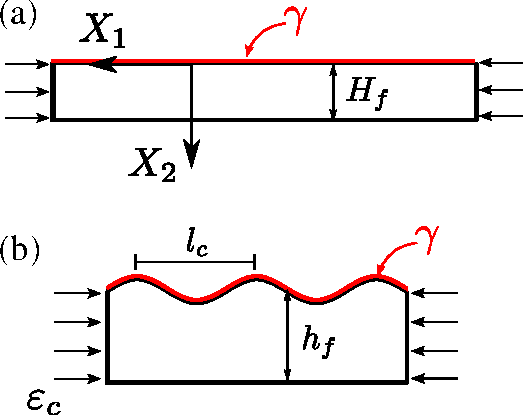
\includegraphics[width=0.78\linewidth]{pics/wrinkle_mech1.pdf}
	\caption{A perfectly flat film subject to compression and surface tension $\gamma$. (a) Undeformed configuration; (b) the formation of wrinkles with wavelength $l_c$. }
	\label{fig:mechfig}
\end{figure}

We first consider a DE film under compression, that is also subject to surface tension effects on its top surface, as illustrated in Figure (\ref{fig:mechfig}). The deformation of the body is described by the field $\mathbf{x}(\mathbf{X})$. The deformation gradient tensor $\mathbf{F}$ is defined as:
\begin{equation}
	\mathbf{F}=\nabla \mathbf{x}
	\label{eq:defgrad1}
\end{equation}
The DE is modeled as an incompressible neo-Hookean material with the free energy density function:
\begin{equation}
	W(\mathbf{F})=\frac{\mu}{2}\mathbf{F} : \mathbf{F}-\pi(\det{\mathbf{F}}-1)
	\label{eq:neoHookean}
\end{equation}
where $\mathbf{A} : \mathbf{B} = \text{tr}(\mathbf{A}^T \mathbf{B})$ denotes the tensor inner product. The first Piola-Kirchhoff (nominal) stress tensor $\mathbf{S}$ can be derived as:
\begin{equation}
	\mathbf{S}=\frac{\partial W(\mathbf{F})}{\partial \mathbf{F}}=\mu\mathbf{F}-\pi \mathbf{F}^{-T}
	\label{eq:mechstress1}
\end{equation}
where $\mu$ is the shear modulus, and $\pi=\pi(\mathbf{X})$ is the Lagrange multiplier to enforce the constraint of incompressibility: $J=\det{\mathbf{F}}=1$. 
The nominal stress satisfies the reference equilibrium equation:
\begin{equation}
	\nabla \cdot \mathbf{S} = \mathbf{0}
	\label{eq:equil_equ}
\end{equation}

On the surface of the body the film is subjected to the Young-Laplace boundary condition~\citep{saksonoCM2006} with surface tension $\gamma$:
\begin{equation}
	\mathbf{S}\mathbf{N}dA=2\gamma\kappa \mathbf{n} da
	\label{eq:YLBC}
\end{equation}
where $\mathbf{N}$ is the unit normal vector to the surface of the body in the undeformed state, $\mathbf{n}$ is the unit normal vector in the current state, and $\kappa$ is the mean curvature of the surface. 

We now add a perturbation into the state of finite deformation with position $\mathbf{x}_{0}(\mathbf{X})$, deformation gradient $\mathbf{F}_{0}(\mathbf{X})$ and nominal stress $\mathbf{S}_{0}(\mathbf{X})$. If the deformation in the $z$-direction is constrained, only 2D plane strain deformation is considered. The background deformation gradient of this state is
\begin{equation}
\mathbf{F}_{0}=
	\begin{bmatrix}
		\lambda & 0  \\
		0 & 1/\lambda \\
	\end{bmatrix}
\end{equation}
Therefore the corresponding base position is $\mathbf{x}_0 = \mathbf{F}_{0}\mathbf{X}$. Now by adding a small displacement perturbation $\delta\mathbf{x}$ and pressure perturbation $\delta\pi$, we write the perturbed state as $\mathbf{x} = \mathbf{x}_{0}(\mathbf{X})+ \delta\mathbf{x}(\mathbf{X})$ and $\pi = \pi_0 + \delta\pi$. Both the base state and the perturbed state satisfy the same governing equations in (\ref{eq:defgrad1}) and (\ref{eq:equil_equ}). The incremental form of the deformation gradient reduces to
\begin{equation}
	\delta\mathbf{F}=\nabla(\delta\mathbf{x})
	\label{eq:defgraddot}	
\end{equation}
and the equilibrium equation to
\begin{equation}
	\nabla \cdot (\delta\mathbf{S}) = \mathbf{0}
	\label{eq:dot_equilbrium}
\end{equation}
where the incremental nominal stress tensor can be obtained using directional differentiation at $\mathbf{F}_{0}$ of the stress in (\ref{eq:mechstress1}):
\begin{equation}
	\delta\mathbf{S}=\mu \delta\mathbf{F} - \delta\pi \mathbf{F}^{-T}_{0} + \pi_{0} \mathbf{F}^{-T}_{0} (\delta\mathbf{F})^T \mathbf{F}^{-T}_{0}
	\label{eq:Sigma_ij}
\end{equation}
Inserting (\ref{eq:Sigma_ij}) into (\ref{eq:dot_equilbrium}) we can obtain the following equation:
\begin{equation}
	\mu \nabla^2 (\delta\mathbf{x}) + \pi_{0} \mathbf{F}^{-T}_{0} \nabla \cdot \left[ (\delta\mathbf{F})^T \mathbf{F}^{-T}_{0} \right] - \mathbf{F}^{-T}_{0} \nabla (\delta\pi) = \mathbf{0}
	\label{eq:dotequil1}
\end{equation}
Taking the directional derivative of the incompressibility condition yields:
\begin{equation}
	\mathbf{F}^{-T}_{0} : \delta\mathbf{F}=0 \implies \frac{1}{\lambda}\frac{\partial(\delta x_1)}{\partial X_1} + \lambda\frac{\partial(\delta x_2)}{\partial X_2} = 0
	\label{eq:icompressdot}
\end{equation}
where the perturbation of the boundary condition reads:
\begin{equation}
	\delta\mathbf{S}\mathbf{N}=2\gamma\delta\kappa\,\mathbf{F}^{-T}_{0}\mathbf{N}
	\label{eq:BC_gamma}
\end{equation}
where the baseline flat state satisfies $\kappa=0$, so the surface tension
contributes only through the curvature increment $\delta\kappa$. The
perturbed surface lives in the \emph{current} configuration, where the
in-plane coordinate is $x_1=\lambda X_1$; its curvature increment is
therefore
\begin{equation}
	\delta\kappa = -\frac{\partial^{2}(\delta x_2)}{\partial x_1^{2}}
	             = -\frac{1}{\lambda^{2}}\frac{\partial^{2}(\delta x_2)}{\partial X_1^{2}}
	             = \frac{K^{2}}{\lambda^{2}}\,f_2(X_2)\cos(K X_1),
	\label{eq:curv_inc}
\end{equation}
the factor $\lambda^{-2}$ arising because the wavelength is stretched by
$\lambda$. The Young--Laplace force $\gamma\,\delta\kappa$ acts per unit
\emph{current} surface area; mapping it back to a nominal traction over the
reference surface introduces the surface stretch (Jacobian)
$\mathrm{d}a/\mathrm{d}A=\lambda$, so the surface tension enters the normal
traction balance as the restoring, stabilizing term
$(\gamma K^{2}/\lambda)\,\delta x_2$. (For a strain-dependent, nominal
surface stress the factor would instead be $1/\lambda$ alone; the two
coincide here because $\gamma$ is the physical residual tension.) At the bottom of the film ($X_2 = H_f$) we impose a constrained-sliding (frictionless roller) base, $t_1=0$ and $f_2=0$, matching the substrate condition of the finite-element model; a bonded base ($f_1=f_2=0$) shifts the onset strain by less than $0.01$ and is not pursued here:
\begin{equation}
	\delta S_{12}=0 \quad \text{and} \quad \delta x_2=0
	\label{eq:BC_bottom1}
\end{equation}

\subsection{Dielectric Elastomer with Surface Tension and Electric Field Effects}

\begin{figure}
	\centering
	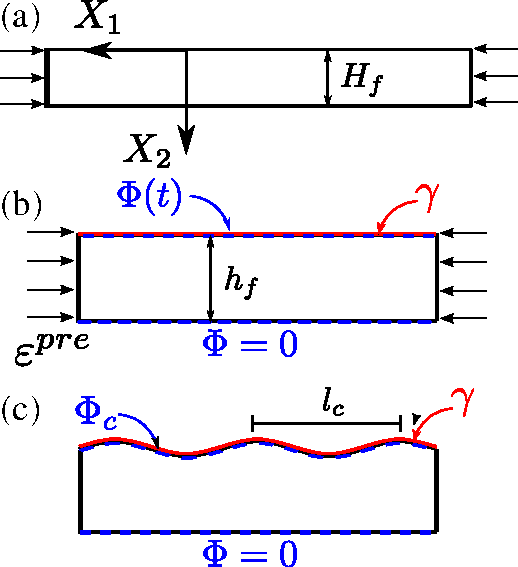
\includegraphics[width=0.78\linewidth]{pics/wrinkle_elec_mech1.pdf}
	\caption{A perfectly flat film subject to compression, electric field and surface tension $\gamma$. (a) Undeformed configuration; (b) Compressed to a given strain $\varepsilon^{pre}$, after which voltage $\Phi(t)$ is applied to the top surface while $\Phi=0$ on the bottom surface; (c) The formation of wrinkles with critical wavelength $l_c$ at critical electric potential $\Phi_c$. }
	\label{fig:elecmechfig}
\end{figure}

We now consider the general problem of interest, that of a DE film that is subject to compressive loading, while accounting for both surface tension and electrostatic loading via electric fields. This is illustrated in Figure (\ref{fig:elecmechfig}). In this case, the reference configuration is a pre-compressed plane strain film, subject to the background deformation gradient $\mathbf{F}_0$ governed by the mechanical pre-stretch $\lambda_{pre}$.

At this state (Figure \ref{fig:elecmechfig}-b), an electric potential $\Phi$ is applied on top of the film along with the surface tension $\gamma$. When the elastomer is at the flat state, the true electric field in the layer is homogeneous, expressed as:
\begin{equation}
	\mathbf{E}=\begin{bmatrix}
	0 \\
	E_2 \\
\end{bmatrix}	
	\label{eq:elecfield} 
\end{equation}
where $E_2=\Phi/h_f$ is the \emph{true} (current-configuration) electric field and $h_f=H_f/\lambda_{pre}$ is the current height of the pre-compressed film. It is convenient to also define the \emph{nominal} field referred to the undeformed thickness, $\tilde E=\Phi/H_f$, which is the directly controlled loading parameter (applied voltage per reference thickness). The two are related through the thickness stretch,
\begin{equation}
	E_2=\frac{\Phi}{h_f}=\frac{\Phi}{H_f/\lambda_{pre}}=\lambda_{pre}\,\tilde E,
	\qquad\text{equivalently}\qquad \tilde E=E_2/\lambda_{pre}.
	\label{eq:Enominal}
\end{equation}
The true field $E_2$ enters the Maxwell stress, whereas the critical thresholds are reported below in terms of the nominal field $\tilde E_c=E_{2,c}/\lambda_{pre}$; in the finite-element model the applied potential is divided by the reference thickness $H_f$, so the code returns $\tilde E$ directly.

The total nominal stress is augmented by the nominal Maxwell electrostatic stress tensor $\mathbf{S}^e$:
\begin{equation}
	\mathbf{S}_{total} = \mathbf{S} + \mathbf{S}^e, \quad \mathbf{S}^e = \det(\mathbf{F}) \boldsymbol{\sigma}^e \mathbf{F}^{-T}
\end{equation}
where $\boldsymbol{\sigma}^e = \epsilon \mathbf{E} \otimes \mathbf{E} - \frac{1}{2}\epsilon |\mathbf{E}|^2 \mathbf{I}$ represents the true spatial Maxwell stress tensor, and $\epsilon$ is the material permittivity. Crucially, enforcing the traction-free boundary condition at the flat top face prior to the onset of wrinkling identifies the background hydrostatic pressure $\pi_0$:
\begin{equation}
	S_{22}^{total, 0} = \left(\frac{\mu}{\lambda_{pre}} - \pi_0 \lambda_{pre}\right) + \frac{1}{2}\lambda_{pre}\epsilon E_2^2 = 0 \implies \pi_0 = \frac{\mu}{(\lambda_{pre})^2} + \frac{1}{2}\epsilon E_2^2
\end{equation}
The mechanical balance $\nabla\cdot\mathbf{S}_{total}=\mathbf{0}$ must now be solved \emph{together} with the incremental Gauss law $\nabla\cdot\delta\tilde{\mathbf{D}}=\mathbf{0}$ for the nominal electric displacement, because the field inside the film is itself perturbed by the incipient wrinkling. Introducing the displacement perturbation $\delta\mathbf{x}$, the constraint-pressure perturbation $\delta\pi$, and the perturbed potential $\delta\phi$ (all referred to the reference frame $\mathbf{X}$), the incremental total stress and electric displacement read
\begin{equation}
	\delta\mathbf{S}_{total} = \mu \delta\mathbf{F} - \delta\pi \mathbf{F}^{-T}_{0} + \pi_{0} \mathbf{F}^{-T}_{0} (\delta\mathbf{F})^T \mathbf{F}^{-T}_{0} + \delta \mathbf{S}^e,
	\qquad
	\delta\tilde{\mathbf{D}}=\epsilon\,\delta\!\left(\mathbf{C}^{-1}\boldsymbol{\mathfrak{E}}\right),
	\label{eq:incr_total}
\end{equation}
where $\boldsymbol{\mathfrak{E}}=-\nabla_{\!X}\phi$ is the referential (nominal) electric field, $\delta\boldsymbol{\mathfrak{E}}=-\nabla_{\!X}\delta\phi$, and $\delta\mathbf{S}^e$ is the increment of the nominal Maxwell stress. Crucially, both $\delta\mathbf{S}^e$ and $\delta\tilde{\mathbf{D}}$ depend on the perturbed potential $\delta\phi$ as well as on $\delta\mathbf{F}$; the bulk electromechanical coupling cannot be reduced to a thickness-gap argument alone.

A central simplification follows once $\delta\phi$ is treated consistently. The compliant electrodes are bonded to the faces and held at fixed voltage, so they remain equipotentials; in the reference frame these faces are flat ($X_2=0,H_f$) and the perturbed potential vanishes there,
\begin{equation}
	\delta\phi(X_1,0)=\delta\phi(X_1,H_f)=0 .
	\label{eq:elec_BC_phi}
\end{equation}
Solving the incremental Gauss law subject to~(\ref{eq:elec_BC_phi}) \emph{slaves} $\delta\phi$ to the displacement field. When this solution is substituted back into the momentum balance, the electric contributions \emph{cancel identically from the bulk}: the through-thickness Maxwell pre-stress (already absorbed into $\pi_0$) and the bulk field perturbation offset one another. The vertical-displacement envelope is therefore governed by the \emph{same} fourth-order equation as the purely mechanical problem~(\ref{eq:ODE_2}), and the electric field does \emph{not} enter the bulk operator. It couples to the wrinkling \emph{only through the boundary conditions}---a structural feature of the incremental electroelasticity of ideal dielectrics that also appears in the independent bifurcation analysis of free-standing dielectric blocks by~\citet{yangJAM2017}, where the field likewise drops out of the bulk equation and survives only in the surface conditions. This corrects the naive treatment, in which retaining $\pi_0$ as an isotropic pressure while discarding the bulk field perturbation produces a spurious field-dependent bulk equation.

On the top face the incremental traction balances the surface tension through the Young--Laplace relation
\begin{equation}
	\delta\mathbf{S}_{total} \mathbf{N} = 2\gamma\delta\kappa \mathbf{F}_0^{-T}\mathbf{N},
	\label{eq:BC_elec_gamma}
\end{equation}
in which $\delta\mathbf{S}_{total}$ now carries the consistent Maxwell traction increment built from the slaved potential. Its physical content is transparent: a surface bulge $\delta x_2$ alters the local gap and hence the field, $\delta E_2=-E_2\,\delta x_2/h_f$, weakening the compressive Maxwell traction where the surface rises and thereby amplifying the perturbation---a destabilizing surface term $\propto\epsilon E_2^2/h_f$ that enters the normal-traction condition below.

At the base we adopt a clamped support, $\delta x_1=\delta x_2=0$ at $X_2=H_f$, which isolates the surface wrinkle:
\begin{equation}
	\delta x_2(X_1,H_f)=0 \quad\text{and}\quad \partial_{X_2}\delta x_2(X_1,H_f)=0 .
	\label{eq:BC_bottom2}
\end{equation}
A sliding (roller) base, $\delta x_2=\delta S_{12}=0$, additionally admits a long-wavelength global mode of the freely sliding layer, whose critical field falls monotonically with wavelength; this mode is cut off by the finite length and end grips of the film---and of the finite-element domain used for validation---so the finite-wavelength wrinkle obtained with the clamped base is the physically operative branch.

\section{Linear Perturbation Analysis for Wrinkles}
\label{AppexB}
\subsection{Compression with elastocapillary effect}

To determine the onset of wrinkling, we look for non-trivial solutions to the eigenvalue problem via Fourier representation:
\begin{equation}
	\begin{aligned}
		\delta x_{1}(X_1,X_2) &= f_{1}(X_2)\sin( K X_1) \\
		\delta x_{2}(X_1,X_2) &= f_{2}(X_2)\cos(K X_1) \\
		\delta \pi(X_1,X_2) &= f_{3}(X_2)\cos(K X_1)
	\end{aligned}
	\label{eq:per_sol}
\end{equation}
Substituting these fields into the mechanical equilibrium lines and eliminating the pressure envelope $f_3(X_2)$ yields the classical fourth-order ordinary differential equation for the vertical envelope function $f_2$:
\begin{equation}
	\frac{\mathrm{d}^4 f_2}{\mathrm{d}X_2^4} - K^2\left(\lambda^{-4}+1\right)\frac{\mathrm{d}^2 f_2}{\mathrm{d}X_2^2} + K^4{\lambda}^{-4}f_2=0
		\label{eq:ODE_2}
\end{equation}
where $K=2\pi/L$ is the reference wavenumber. The general solution represents an exponential expansion system $\mathbf{A}\mathbf{C} = \mathbf{0}$, requiring:
\begin{equation}
	\det \mathbf{A}=0
	\label{eq:eig_1}
\end{equation}
The correct, balanced matrix entries for $\mathbf{A}$ are given as follows:
\begin{equation}
\begin{aligned}
	A_{11} &= -\frac{\gamma  K^2 H_f}{\lambda \mu }- H_f K\left(\lambda^2  +\frac{  1}{\lambda ^2}\right), & A_{12} &= -\frac{\gamma  K^2 H_f}{\lambda \mu }+ H_f K\left(\lambda^2  +\frac{  1}{\lambda ^2}\right) \\
	A_{13} &= -\frac{\gamma K^2 H_f}{\mu \lambda }-2 KH_f, & A_{14} &= -\frac{\gamma K^2 H_f}{\mu \lambda }+2 KH_f   \\
	A_{21} &= A_{22}=\frac{2 K H_f}{\lambda ^2}, & A_{23} &= A_{24}= \lambda ^2 K H_f+\frac{K H_f}{\lambda ^2}
\end{aligned}
\end{equation}
\begin{equation}
	\begin{aligned}
	A_{31} &=\frac{2 K H_f \,e^{-K H_f {\lambda ^{-2}}}}{\lambda ^2}, & A_{32} &=\frac{2 K H_f \,e^{K H_f {\lambda ^{-2}}}}{\lambda ^2} \\
	A_{33} &=\left(\lambda ^2 K H_f + \frac{K H_f}{\lambda^2}\right) e^{-K H_f}, & A_{34} &=\left(\lambda ^2 K H_f + \frac{K H_f}{\lambda^2}\right) e^{K H_f} \\
	A_{41} &=e^{-{K H_f}{\lambda ^{-2}}}, \quad A_{42}=e^{{K H_f}{\lambda ^{-2}}}, & A_{43} &=e^{-K H_f}, \quad A_{44}=e^{K H_f}
	\end{aligned}
\end{equation}

By solving the eigenvalue problem in (\ref{eq:eig_1}), we obtain the relation between stretch $\lambda$, and compressive strain $\varepsilon=1-\lambda$ with the wavelength $l$ (Figure \ref{fig:mechfig_plot}). 

\begin{figure}
	\centering
	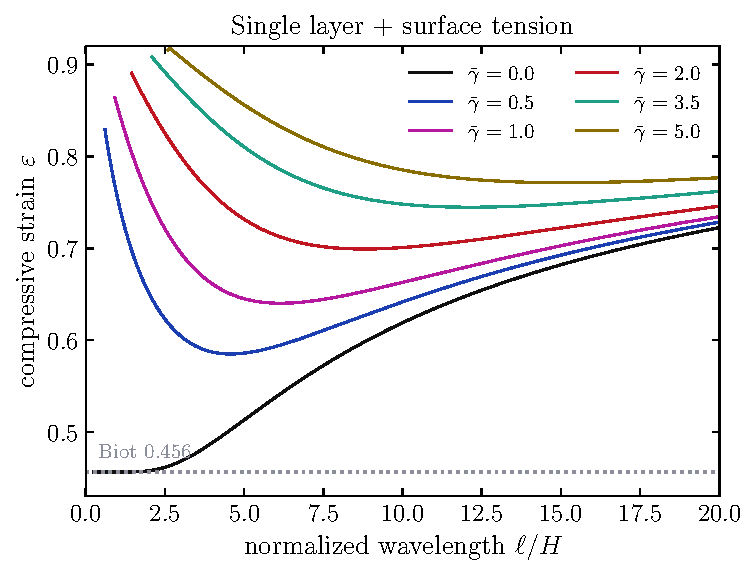
\includegraphics[width=0.72\linewidth]{pics/ew_mech.pdf}
	\caption{Strain vs. wavelength for a range of elastocapillary numbers}
	\label{fig:mechfig_plot}
\end{figure}

When surface tension is neglected ($\gamma=0$), we recover Biot's value of wrinkling at $\varepsilon_{w}\approx0.46$ as shown in Figure \ref{fig:mechfig_plot}~\citep{Biot1963}. When surface tension is present ($\gamma>0$), the strain $\varepsilon$ first decreases and then increases as the normalized wavelength $l/H_f$ increases (Figure \ref{fig:mechfig_plot}). The key effect of surface tension is that it inhibits bifurcation, as both the critical strain $\varepsilon_c$ and corresponding normalized wavelength $l_c/H_f$ increase with increasing $\gamma/(\mu H_f)$ (Figure \ref{fig:mechfig_plot_fem}). 

In addition, although the critical strain rises steeply at small elastocapillary numbers and appears to level off over the range plotted, it does \emph{not} saturate at a finite value: as $\gamma/(\mu H_f)\to\infty$ the residual decays algebraically, $1-\varepsilon_c\sim(\gamma/\mu H_f)^{-1/3}$, so that $\varepsilon_c\to1$ (full compression) while the selected wavelength $l_c/H_f$ grows without bound. The steepest rise occurs at small elastocapillary numbers: $\varepsilon_c$ increases by more than $34\%$ from $0.46$ at $\gamma/(\mu H_f)=0$ to ${\approx}0.70$ at $\gamma/(\mu H_f)=2$, and thereafter more gradually---${\approx}0.77$ at $\gamma/(\mu H_f)=5$---consistent with the slow $\bar\gamma^{-1/3}$ approach to unity (Figure \ref{fig:mechfig_plot_fem}a).

\begin{figure}
	\centering
	\begin{subfigure}[b]{0.5\textwidth}
		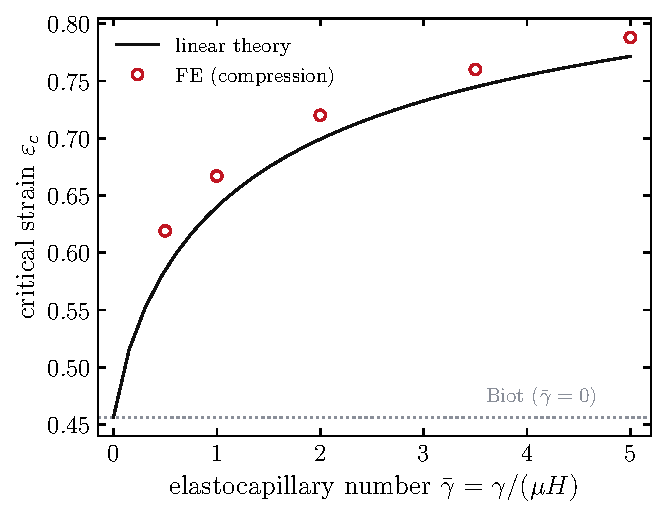
\includegraphics[width=\linewidth]{pics/ge_mech.pdf}
		\caption{}
	\end{subfigure}
	\begin{subfigure}[b]{0.5\textwidth}
		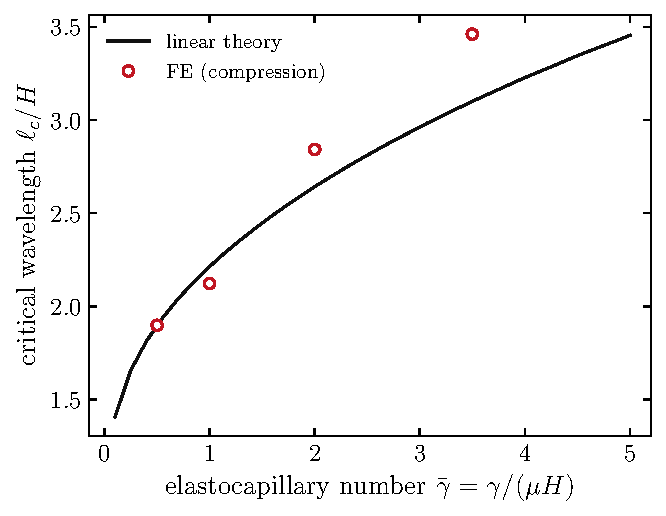
\includegraphics[width=\linewidth]{pics/gl_mech.pdf}
		\caption{}
	\end{subfigure}
	\caption{(a) Critical strain $\varepsilon_c$ and (b) critical wavelength $l_c/H_f$ (the \emph{current}, deformed crest-to-crest spacing) versus elastocapillary number $\gamma/(\mu H_f)$, for an incompressible neo-Hookean film on a frictionless (roller) base. Solid lines are the linear-perturbation prediction; markers are nonlinear FE results obtained by undamped symmetric compression---the onset strain (a) lies within ${\sim}6\%$ of theory and the wavelength (b) within ${\sim}12\%$ for $\bar\gamma\leqslant3.5$ (the $\bar\gamma=5$ point is omitted, being quantization-limited to two periods on the finite strip). The dashed line marks the Biot threshold $\varepsilon_c\approx0.456$ recovered as $\gamma\to0$; neither quantity saturates---as $\bar\gamma\to\infty$, $\varepsilon_c\to1$ with $1-\varepsilon_c\sim\bar\gamma^{-1/3}$ while $l_c/H_f$ keeps growing.}
	\label{fig:mechfig_plot_fem}
\end{figure}

We verify the perturbation predictions with dynamic, nonlinear finite-element (FE) calculations using the open-source code~\citet{tahoe} with 4-node bilinear quadrilateral plane-strain elements in a mean-dilatation (Q1P0) formulation for near-incompressibility. A film of thickness $H_f=4$ (element size $0.5$) is compressed \emph{symmetrically} under displacement control: both ends are driven inward equally on a frictionless roller base ($t_1=0,\,f_2=0$, the same substrate condition as the perturbation analysis), so the homogeneous compression stays uniform and free of any loaded-edge bias, while the Young--Laplace traction acts on the deforming top surface. The explicit central-difference march is kept quasi-static by mild mass scaling and, for the reason given below, run without artificial damping; no geometric imperfection is seeded, so the instability grows from numerical noise. The unseeded bifurcation is sharp---the surface amplitude jumps from the noise floor to $O(H_f)$ over a narrow strain window---so the onset strain is identified as the point where the amplitude first exceeds a small threshold above the noise (approaching the Biot value $\varepsilon_c\approx0.456$ as $\bar\gamma\to0$), and the wavelength is read from the peak of the zero-padded Fourier spectrum of the deformed top surface at that frame.

The simulations span the surface-tension--dominated regime $\bar\gamma=\gamma/(\mu H_f)=0.5,\,1,\,2,\,3.5,\,5$, where surface tension suppresses the competing crease (Section~\ref{sec:crease_wrinkle}) and the smooth wrinkle is the first instability the FE resolves. As shown in Figure~\ref{fig:mechfig_plot_fem}(a), the FE onset strains track the predicted $\varepsilon_c(\bar\gamma)$ closely, $\varepsilon_c^{\rm FE}=0.62,\,0.67,\,0.72,\,0.76,\,0.79$ against the theoretical $0.59,\,0.64,\,0.70,\,0.75,\,0.77$---within ${\sim}6\%$, the expected offset between an infinitesimal-amplitude bifurcation and a finite-amplitude, dynamically seeded onset. The agreement is moreover scale-invariant: doubling both $L_f$ and $H_f$ at fixed $\bar\gamma$ reproduces the dimensionless $\varepsilon_c(\bar\gamma)$ to within a fraction of a percent, confirming that the FE captures the intrinsic instability rather than a mesh- or domain-set artifact.

Figure~\ref{fig:mechfig_plot_fem}(b) reports the \emph{current} (deformed) wrinkle spacing $l_c$---the crest-to-crest distance measured on the compressed film, related to the referential wavelength by $l_c=(1-\varepsilon_c)\,2\pi/K_c$. Two aspects of the finite-element setup control its fidelity. First, the explicit march is run \emph{without} artificial damping: with damping the incipient wrinkle localizes against the loaded ends (a Saint-Venant boundary layer), whereas the undamped dynamics let it develop uniformly across the interior, so the measured spacing reflects the intrinsic wrinkle rather than an edge effect. Second, resolving a clean wave train demands enough periods within the domain: the number of wrinkles $N\simeq L_f/l_{\rm ref}$ is set by the referential wavelength $l_{\rm ref}=l_c/(1-\varepsilon_c)$, so at $\bar\gamma=5$ ($l_{\rm ref}\approx15H_f$) a strip of $L_f\gtrsim45H_f$ is needed for three periods. On the $L_f=180,\,H_f=4$ strip used here the FE wavelengths track the prediction to within ${\sim}12\%$ for $\bar\gamma\leqslant3.5$; at $\bar\gamma=5$ the domain accommodates only two periods rather than three, so that point is quantization-limited and is omitted. The onset strain, reproduced to ${\sim}6\%$ across film sizes, remains the more robust comparison.

\begin{figure}
	\centering
	\figplaceholder{pics/wrinkle_mech_fe.pdf}
\caption{Results for FE simulation of a mechanical compression-induced instability of an $40\times4$ elastomer film. (a) Undeformed film (b) Onset of wrinkling instability on the top surface at the critical strain $\varepsilon_c=0.547$ and elastocapillary number $\gamma/(\mu H_f)=0.2$. _D_VEC is the displacement magnitude.}
	\label{fig:fem_s12}
\end{figure}

\subsection{Scope: wrinkling versus creasing}
\label{sec:crease_wrinkle}

The perturbation analysis above describes \emph{wrinkling}: a supercritical, smoothly undulating bifurcation of the flat surface that for a traction-free neo-Hookean half-space recovers the Biot threshold $\varepsilon_{w}\approx0.46$ ($\lambda_w\approx0.54$). We note that a free soft surface under compression is also susceptible to \emph{creasing}, a strongly nonlinear, subcritical and essentially scale-free instability in which the surface folds into localized self-contact, nucleating at a lower strain $\varepsilon_{cr}\approx0.35$ in the absence of surface tension~\citep{hong2009formation,jin2014creases,cai2012creasing,hong2013crease}.

We deliberately restrict the present study to wrinkling, for three reasons. First, creasing is a finite-amplitude instability with no intrinsic wavelength and is therefore inaccessible in principle to an infinitesimal-amplitude perturbation analysis. The perturbation theory presumes a characteristic wavelength $L\propto1/K$, whereas the crease is effectively a singular, vanishing-wavelength fold ($K\to\infty$). Surface tension does impose a cutoff length scale $\ell_{\rm cutoff}\sim\gamma/\mu$ below which the surface-energy cost of curvature is prohibitive, so that features sharper than $\ell_{\rm cutoff}$ are penalized; but this regularizes rather than removes the singular nature of the crease, whose onset and morphology still require a fully nonlinear treatment with surface self-contact---a distinct methodology outside the scope of the linear framework developed here. Second, surface tension acts strongly against the crease: because a crease is a region of very high surface curvature, its formation carries a surface-energy penalty that scales with the local curvature and thus penalizes the sharp, short-wavelength fold far more than the smooth, long-wavelength wrinkle~\citep{chenPRL2012}. Consequently, in the surface-tension--dominated regime of moderate-to-large elastocapillary number---precisely the regime targeted in this work---wrinkling is the first instability encountered, and the linear prediction is the physically operative one. Third, the engineering interest in actuated dielectric-elastomer laminates lies in the recoverable, periodic wrinkle morphology rather than the hysteretic crease. A quantitative determination of the crease--wrinkle crossover, which would require nonlinear self-contact simulation, is left to future work.

\subsection{Compressed film subject to surface tension and electric field}

Substituting the Fourier ansatz~(\ref{eq:per_sol}) into the coupled incremental equations and eliminating both the constraint pressure and---through the slaved electrostatics established above---the perturbed potential, the electric field cancels from the bulk and the vertical envelope obeys the \emph{purely mechanical} equation~(\ref{eq:ODE_2}),
\begin{equation}
	\frac{\mathrm{d}^4 f_2}{\mathrm{d}X_2^4} - K^2\!\left(\lambda_{pre}^{-4}+1\right)\frac{\mathrm{d}^2 f_2}{\mathrm{d}X_2^2} + K^4\lambda_{pre}^{-4}\, f_2 = 0 ,
	\label{eq:ODE_3}
\end{equation}
with characteristic roots the mechanical exponents
\begin{equation}
	q=\pm K,\ \pm K/\lambda_{pre}^{2},
	\qquad
	f_2(X_2)=\sum_{i=1}^{4}c_i\,e^{q_i X_2},
	\label{eq:elec_roots}
\end{equation}
\emph{independent of the electric field}. This is an exact statement, not an $E_2\to0$ approximation: solving the incremental Gauss law for $\delta\phi$ and substituting back removes every field term from the bulk operator, so the characteristic polynomial factors as $(q^2-K^2)(\lambda_{pre}^{4}q^2-K^2)=0$ for all $E_2$. The electric loading is felt entirely through the boundary conditions.

The four amplitudes $c_i$, together with the slaved potential, are fixed by the boundary conditions. At the clamped base the displacement vanishes,
\begin{equation}
	f_2(H_f)=0,\qquad f_2'(H_f)=0,
\end{equation}
while at the free top surface the tangential traction vanishes and the normal traction balances the surface tension and the linearized Maxwell pressure,
\begin{equation}
	\delta S_{12}=0,\qquad
	\delta S_{22}^{total} + \frac{\gamma K^2}{\lambda_{pre}}\,\delta x_2
	- \frac{\lambda_{pre}^2\,\epsilon E_2^2}{H_f}\,\delta x_2 = 0,
	\label{eq:elec_topBC}
\end{equation}
with the surface-tension term $\gamma K^2/\lambda_{pre}$ stabilizing and the Maxwell term $\lambda_{pre}^2\epsilon E_2^2/H_f=\lambda_{pre}\,\epsilon E_2^2/h_f$ ($h_f=H_f/\lambda_{pre}$) destabilizing. Both surface tractions enter the \emph{nominal} balance referred to the reference area: the physical (current-area) Maxwell traction $\epsilon E_2^2/h_f$ and the Young--Laplace traction $\gamma K_{\rm cur}^2=\gamma(K/\lambda_{pre})^2$ are each multiplied by the in-plane area stretch $\lambda_{pre}$, giving $\lambda_{pre}^2\epsilon E_2^2/H_f$ and $\gamma K^2/\lambda_{pre}$ respectively. Here $\delta S_{12}$ and $\delta S_{22}^{total}$ are the incremental tractions built from $f_1=-(\lambda_{pre}^2/K)f_2'$, the slaved potential, and the field-augmented base pressure $\pi_0=\mu/\lambda_{pre}^2+\tfrac12\epsilon E_2^2$. Imposing these four conditions on~(\ref{eq:elec_roots}) yields a homogeneous system $\mathbf{B}(\lambda_{pre},K,E_2)\,\mathbf{c}=\mathbf{0}$ whose top-row entries carry the electric coupling---through the slaved potential and the surface Maxwell traction---and which reduces to the mechanical boundary matrix $\mathbf{A}$ as $E_2\to0$. Nontrivial solutions require
\begin{equation}
	\det\mathbf{B}=0 .
	\label{eq:elec_det}
\end{equation}
As $E_2\to0$ the coupling vanishes and~\eqref{eq:elec_det} coincides with the mechanical criterion $\det\mathbf{A}=0$, recovering the Biot threshold; we have verified this numerically ($\varepsilon_c=0.456$ at $\gamma=E_2=0$). Minimizing $\det\mathbf{B}=0$ over the wavenumber $K$ gives the critical normalized nominal field $\tilde{E}_c\sqrt{\epsilon/\mu}$, shown in Figures~\ref{fig:e2_elec} and~\ref{fig:e2_elec_stretch} for a pre-compressed ($\lambda_{pre}=0.9$) and a pre-stretched ($\lambda_{pre}=1.2$) film, respectively.

\begin{figure}
	\centering
	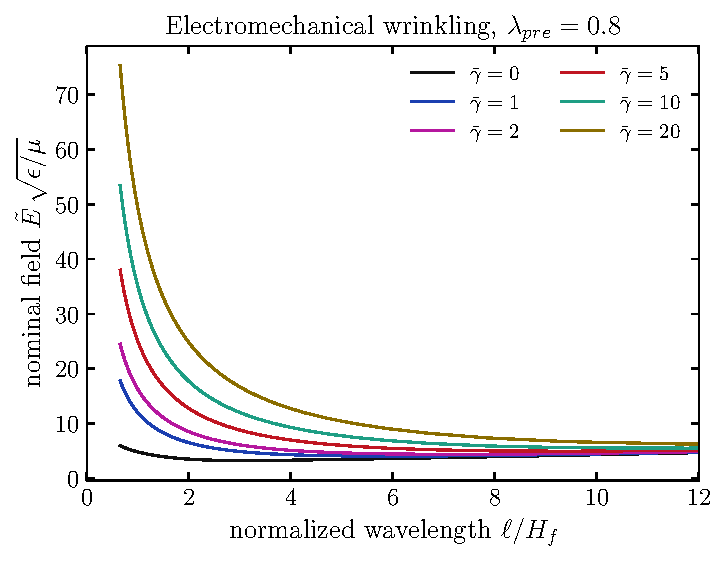
\includegraphics[width=0.72\linewidth]{pics/e2_elec.pdf}
	\caption{Electromechanical neutral-stability curves (perturbation analysis) at pre-compression $\lambda_{pre}=0.9$ ($\varepsilon^{pre}=0.1$): normalized nominal electric field $\tilde E\sqrt{\epsilon/\mu}$ versus normalized wavelength $\ell/H_f$ for several elastocapillary numbers $\gamma/(\mu H_f)$. The critical field is the minimum of each curve, which rises and moves to longer wavelength as surface tension increases (Figure~\ref{fig:lam1_compare}).}
	\label{fig:e2_elec}
\end{figure}

\begin{figure}
	\centering
	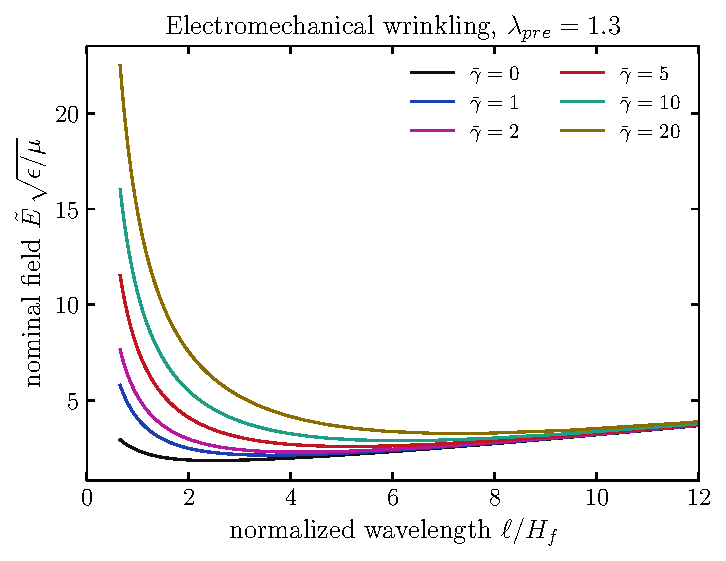
\includegraphics[width=0.72\linewidth]{pics/e2_elec_stretch.pdf}
	\caption{The same electromechanical neutral-stability curves at pre-\emph{stretch} $\lambda_{pre}=1.2$. As in the pre-compressed case, increasing surface tension raises the critical field and lengthens the selected wavelength; the absolute fields are uniformly lower than at $\lambda_{pre}=0.9$ (Figure~\ref{fig:e2_elec}) because the thinner pre-stretched film reaches a given true field $E_2=\lambda_{pre}\tilde E$ at a smaller applied voltage.}
	\label{fig:e2_elec_stretch}
\end{figure}

In the limit of vanishing electric field the criterion reduces to the purely mechanical result of Section~\ref{sec:crease_wrinkle}, recovering the Biot threshold (verified numerically, $\varepsilon_c=0.456$). For $\lambda_{pre}=1$, minimizing $\det\mathbf{B}=0$ over $K$ gives a critical field that grows monotonically with surface tension, $E_c\sqrt{\epsilon/\mu}=2.50,\,2.79,\,2.96,\,3.19,\,3.62,\,4.04,\,4.57$ for $\gamma/(\mu H_f)=0,\,0.5,\,1,\,2,\,5,\,10,\,20$, with the selected wavelength lengthening from $\ell\approx3H_f$ to $\ell\approx10H_f$ (Figure~\ref{fig:lam1_compare}). The growth is asymptotically $\propto\sqrt{\gamma/(\mu H_f)}$: surface tension penalizes the curved deformed surface, so a larger Maxwell traction---hence a higher field---is needed to overcome it, and the penalty is relieved by selecting a longer, gentler wavelength.

The perturbation criterion describes the smooth, infinitesimal-amplitude \emph{wrinkle}. Our nonlinear finite-element simulations (Figure~\ref{fig:lam1_compare}, markers) instead capture the \emph{crease}: a localized, finite-amplitude fold that, being subcritical, nucleates at a \emph{lower} field than the smooth bifurcation. The FE onsets therefore sit $8$--$18\%$ below the perturbation curve across $\gamma/(\mu H_f)\in[0.5,20]$. The two share the same $\sqrt{\gamma}$ growth, but the FE-selected wavelength saturates at $\ell\approx2.5H_f$---the intrinsic scale of a localized fold---while the wrinkle wavelength grows to $\ell\approx10H_f$; the surface deformation in the FE is correspondingly localized rather than sinusoidal. This crease-to-wrinkle offset is the central reason the linear theory and the FE do not coincide; we examine its origin, and rule out numerical causes, in Section~\ref{sec:em_mismatch}.

\begin{figure}
	\centering
	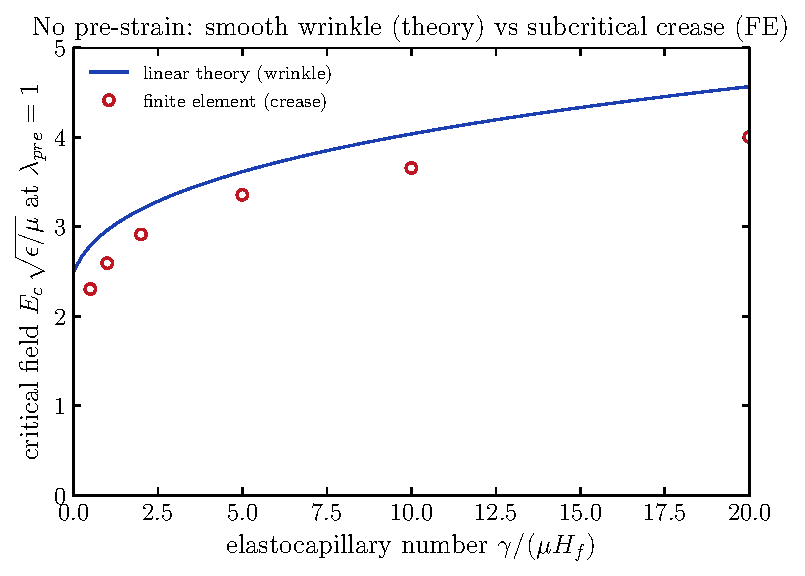
\includegraphics[width=0.7\linewidth]{pics/lam1_compare.pdf}
	\caption{No pre-strain ($\lambda_{pre}=1$): critical nominal field $E_c\sqrt{\epsilon/\mu}$ versus elastocapillary number $\gamma/(\mu H_f)$, extended to $\gamma/(\mu H_f)=20$. The linear perturbation criterion (solid line) gives the smooth wrinkle threshold, which grows as $\sqrt{\gamma/(\mu H_f)}$. Nonlinear finite-element onsets (markers) lie below it: the FE resolves the subcritical crease, which nucleates before the smooth wrinkle. The gap narrows as surface tension suppresses the crease.}
	\label{fig:lam1_compare}
\end{figure}

We next examine the dependence on pre-strain, sweeping from pre-compression $\lambda_{pre}=0.8$ to pre-stretch $\lambda_{pre}=1.3$ at fixed $\gamma/(\mu H_f)=2$. The instability is triggered by the \emph{true} field $E_2$, whose critical value is nearly independent of pre-strain---in the perturbation theory it varies by only ${\sim}10\%$ over $\lambda_{pre}\in[0.8,1.3]$, and in the FE it is constant to within a few percent (Figure~\ref{fig:em_validation}b)---because the local Maxwell stress $\tfrac12\epsilon E_2^2$ must overcome the shear modulus $\mu$, which the pre-strain leaves unchanged. The controlled \emph{nominal} field $\tilde E=\Phi/H_f$ therefore follows the kinematic relation $E_2=\lambda_{pre}\tilde E$: a pre-stretched, hence thinner, film ($h_f=H_f/\lambda_{pre}$) reaches the critical true field at a smaller applied voltage, so $\tilde E_c$ \emph{decreases} with pre-stretch and \emph{increases} with pre-compression (Figure~\ref{fig:em_validation}a). Theory and FE exhibit the \emph{same} pre-strain trend: the nominal threshold falls monotonically with pre-stretch while the true threshold stays nearly flat. This kinematic, uniaxial plane-strain mechanism is distinct from the equibiaxial electromechanical (pull-in) instability~\citep{zhaoAPL2007,keplingerPNAS2010}, in which in-plane pre-stretch stiffens the film against homogeneous thinning.

\begin{figure}
	\centering
	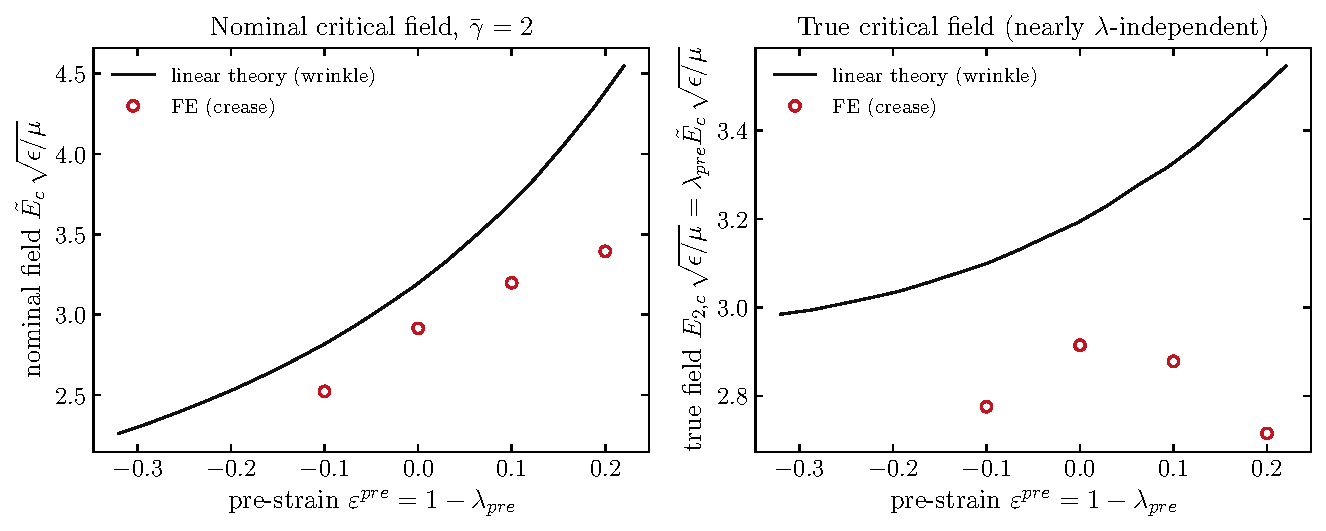
\includegraphics[width=\linewidth]{pics/em_validation.pdf}
	\caption{Pre-strain dependence at $\bar\gamma=2$: finite element (markers) and perturbation theory (line), swept from pre-compression $\lambda_{pre}=0.8$ to pre-stretch $\lambda_{pre}=1.3$. (a) The nominal critical field $\tilde E_c\sqrt{\epsilon/\mu}$ rises with pre-compression and falls with pre-stretch. (b) The true field $E_{2,c}=\lambda_{pre}\tilde E_c$ is nearly $\lambda$-independent (FE to within a few percent; theory to within ${\sim}10\%$), the signature of the kinematic-thinning mechanism. The constant vertical offset between FE and theory is the crease-to-wrinkle gap of Figure~\ref{fig:lam1_compare}.}
	\label{fig:em_validation}
\end{figure}

\subsection{Why the finite-element model and the linear theory disagree}
\label{sec:em_mismatch}

The perturbation criterion and the finite-element onsets share the same trends---the $\sqrt{\gamma/(\mu H_f)}$ growth of the critical field and the kinematic pre-strain dependence---yet the FE thresholds lie $8$--$18\%$ below the theory. The natural question is whether this offset is a numerical artifact of the FE (mesh resolution, explicit dynamics, finite-amplitude detection) or a genuine difference in the instability being captured. Targeted tests show it is the latter: the FE resolves a subcritical \emph{crease}, while the linear analysis is restricted to the smooth \emph{wrinkle}.

\emph{The instability is a crease, not a wrinkle.} Three diagnostics identify the FE mode as a localized, subcritical fold rather than a smooth wave. First, the onset is essentially discontinuous: as the field is ramped, the top-surface amplitude jumps from $0.05H_f$ to $0.5H_f$ over a field increment $\Delta\tilde E\sqrt{\epsilon/\mu}\approx0.03$, less than $1.5\%$ of the threshold---an explosive growth characteristic of a subcritical bifurcation, not the gradual $\sqrt{E-E_c}$ rise of a supercritical wrinkle. Second, the recorded onset field is independent of the amplitude threshold used to define it (the same value at $0.1H_f$, $0.2H_f$, and $0.3H_f$), confirming the jump. Third, the deformed surface at onset is spatially localized: its peak-to-r.m.s.\ ratio is $\approx2.2$ and its participation ratio $\approx0.4$, versus $1.41$ and $\approx0.67$ for a pure sinusoid. A linear, infinitesimal-amplitude theory cannot represent such a scale-free fold, so a downward offset of the FE relative to the wrinkle prediction is expected. Consistently, the FE-selected wavelength saturates at $\ell\approx2.5H_f$ for all $\gamma/(\mu H_f)$, whereas the wrinkle wavelength grows without bound.

\emph{Mesh resolution is not the cause.} Refining the through-thickness discretization fourfold, from $4$ to $16$ elements across the film (mesh $80\times16$), changes the onset field by less than $1\%$: $\tilde E_c\sqrt{\epsilon/\mu}=2.30,\,2.59,\,2.92$ at $\gamma/(\mu H_f)=0.5,1,2$, against $2.31,\,2.60,\,2.91$ on the baseline $80\times4$ mesh. The onset is mesh-converged, so the offset is not an under-resolution effect.

\emph{Dynamic effects do not cause the offset---they oppose it.} Because the FE uses an explicit, ramped quasi-static loading, we tested the sensitivity of the onset to the ramp rate at $\gamma/(\mu H_f)=1$, $\lambda_{pre}=1$. Halving and doubling the rate gives onset fields $\tilde E_c\sqrt{\epsilon/\mu}=2.91$ (fast), $2.60$ (base), $2.39$ (slow): a \emph{faster} ramp raises the apparent onset, because the localizing fold has less time to develop before the field passes the bifurcation. Dynamic and finite-rate effects therefore push the FE onset \emph{upward}, toward the wrinkle prediction; the more quasi-static the simulation, the further the onset falls below the theory. Dynamics thus cannot explain the gap---they have the wrong sign---and the genuinely quasi-static crease threshold lies even lower than the values reported here.

\emph{Summary.} The mesh is converged and dynamics act against the offset, so neither is responsible. The linear theory furnishes the upper, smooth-wrinkle branch with the correct scaling in surface tension and pre-strain; the FE resolves the lower, subcritical crease branch. The two are different instabilities of the same film, and together they bracket the field at which the surface will destabilize. (In real devices the observed field is lower still: surface imperfections nucleate creasing prematurely, and viscoelasticity, electrode compliance, and the uncertain surface energy of a soft solid in fluid all shift the recorded onset.)

\section{Conclusions}

We have presented a linear stability analysis, verified with nonlinear finite-element calculations, for the surface instabilities of dielectric elastomers subject to surface tension. Surface tension is found to significantly affect the wrinkling instability, both raising the critical strain (or electric field) required to trigger it and increasing the selected wavelength. We restricted the analysis to wrinkling and discussed why, in the surface-tension--dominated regime of interest, the competing subcritical crease---which the present infinitesimal-amplitude theory cannot resolve and which surface tension preferentially suppresses---is not the operative instability; its quantitative treatment is left to future work. Surface tension thus emerges as an independently tunable control over the onset and morphology of surface instabilities in dielectric-elastomer actuators operating in fluidic environments.

\section{Acknowledgements}

HSP and SS acknowledge funding from the ARO, grant W911NF-14-1-0022.

\bibliography{biball,park_holmes_nsf_2016}

\end{document}